\documentclass[11pt,a4paper]{article}

% ---------------------------------------------------------------------------
% Observational Response Surfaces versus Interventional Policy
% Master document. Compile with: bash compile.sh   (or: make)
% ---------------------------------------------------------------------------

\usepackage[margin=1in]{geometry}
\usepackage{amsmath,amssymb,amsthm}
\usepackage{booktabs}
\usepackage{multirow}
\usepackage{graphicx}
\usepackage{subcaption}
\usepackage{microtype}
\usepackage{xcolor}
\usepackage[numbers,sort&compress]{natbib}
\usepackage[colorlinks=true,linkcolor=blue!50!black,citecolor=green!40!black,urlcolor=blue!60!black]{hyperref}
\usepackage[capitalise,noabbrev]{cleveref}

\graphicspath{{figures/}}

% ---- theorem environments (for the analytical Pareto derivation) ----------
\theoremstyle{plain}
\newtheorem{lemma}{Lemma}
\newtheorem{theorem}{Theorem}
\newtheorem{corollary}{Corollary}
\theoremstyle{definition}
\newtheorem{definition}{Definition}
\theoremstyle{remark}
\newtheorem{remark}{Remark}

% ---- convenience macros ---------------------------------------------------
\newcommand{\ugm}{\ensuremath{\mu\mathrm{g\,m^{-3}}}}
\newcommand{\ppb}{\ensuremath{\mathrm{ppb}}}
\newcommand{\RR}{\mathbb{R}}
\newcommand{\Exp}{\mathbb{E}}
\newcommand{\zvec}{\mathbf{z}}
\newcommand{\bmat}{\mathbf{B}}
\newcommand{\evec}{\mathbf{e}}

\title{\bfseries Observational Response Surfaces versus Interventional Policy:\\
A Critical Audit of Causal Discovery and Multi-Objective Optimization\\
Across Indian Urban Air Quality Networks}

\author{%
  S.~Krishiykeishav\,$^{1}$ \and Pratyush Amit Sharma\,$^{2}$ \and
  Shreerag Venugopalan Nair\,$^{3}$ \and Jayshil Vinodbhai Prajapati\,$^{4}$ \and
  Ryan Vinod\,$^{5}$ \\[6pt]
  \normalsize Vellore Institute of Technology (VIT), Vellore, Tamil Nadu, India \\[3pt]
  \footnotesize $^{1}$26BME0561, Mech.\ Engg. \quad
  $^{2}$26BCM0060, Chem.\ Engg. \quad
  $^{3}$26BEC0114, ECE \\[1pt]
  \footnotesize $^{4}$26BCE2435, CSE (Core) \quad
  $^{5}$26BCB0026, CSE (Bioinformatics)%
}

\date{\today}

\begin{document}
\maketitle

\begin{abstract}
\noindent
The uncritical application of machine learning and multi-objective optimization to
ambient air-quality telemetry can produce spurious, policy-shaped conclusions,
because non-linear atmospheric chemistry and strong spatio-temporal autocorrelation
violate the assumptions on which naive pipelines rest. We audit a complete
prediction-to-policy pipeline built on $204$ continuous ambient monitoring stations
across urban India---$1{,}180{,}551$ station-hours of criteria pollutants
(PM\textsubscript{2.5}, PM\textsubscript{10}, NO, NO\textsubscript{2},
SO\textsubscript{2}, CO, O\textsubscript{3}) over calendar year 2025, merged with
collocated Open-Meteo reanalysis meteorology---and report three findings. First,
spatio-temporal autocorrelation inflates apparent skill under random row splitting:
contemporaneous ozone estimation attains $R^2 \approx 0.41$ under an i.i.d.\ random
split but only $R^2 \approx 0.25$ under a strict blocked temporal (Q4) holdout and
$R^2 \approx 0.30$ under spatial leave-stations-out validation, while a previous-hour
persistence baseline reaches $R^2 \approx 0.79$; pollutants contribute only
$\Delta R^2 \approx +0.12$ beyond meteorology. Second, linear structural discovery
(DirectLiNGAM) recovers a single bootstrap-stable, meteorology-robust edge consistent
with \emph{localized} nitric-oxide titration ($\mathrm{NO}+\mathrm{O_3}\rightarrow
\mathrm{NO_2}+\mathrm{O_2}$) rather than any regional photochemical-smog mechanism,
a limitation sharpened by the structural absence of volatile organic compounds
(VOCs) and by an authoritative unit audit showing CO, NO\textsubscript{2} and
SO\textsubscript{2} are reported in mixed ppb/\ugm{} units with no per-record
provenance. Third, we prove analytically that over the linear response surface the
true Pareto frontier collapses to a one-dimensional segment, against which
$100\%$ of the heuristic NSGA-II candidate policies are dominated (generational
distance $=0.084$; hypervolume error $=6.6\%$). We reframe the artifact as an
\emph{open, leakage-safe benchmark} and propose a four-part scientific
identification gate for observational environmental AI.

\medskip
\noindent\textbf{Keywords:} air quality; data leakage; causal discovery;
DirectLiNGAM; multi-objective optimization; Pareto dominance; source apportionment;
reproducible benchmark; India.
\end{abstract}


\section{Introduction}
\label{sec:intro}

Urban air pollution is among the most severe environmental health burdens in South
Asia. Rapid urbanization and motorization across the Indo-Gangetic Plain and the
peninsular metropolitan corridors have driven chronic and widespread exceedances of
the National Ambient Air Quality Standards (NAAQS), with annual-mean fine particulate
matter (PM\textsubscript{2.5}) across many Indian cities exceeding national limits by
large multiples and the World Health Organization guideline by an order of magnitude
\citep{guttikunda2013delhi,pant2015delhi}. The expansion of the Continuous Ambient Air
Quality Monitoring Station (CAAQMS) network operated under the Central Pollution
Control Board, together with open aggregation platforms such as OpenAQ \citep{openaq},
has made hourly, multi-pollutant telemetry available at a national scale. This
abundance of observational data has, in turn, invited an increasingly ambitious class
of data-driven analyses that chain together three steps: \emph{prediction} of ambient
concentrations, \emph{discovery} of a causal structure among pollutants, and
\emph{optimization} of ``policies'' framed as pollutant reductions.

\subsection{Mechanistic models versus observational learning}
Two methodological traditions sit in tension. Chemical transport models (CTMs) encode
the governing physics and chemistry of the atmosphere and can, in principle, answer
genuinely interventional questions---what happens to concentrations if a given
emission sector is curtailed. In practice their skill is bounded by bottom-up emission
inventories that are frequently incomplete, out of date, or spatially mis-resolved,
particularly over rapidly changing Indian source regions \citep{guttikunda2013delhi}.
Observational machine learning inverts this trade-off: methods such as gradient-boosted
trees \citep{chen2016xgboost} and random forests \citep{breiman2001rf} excel at fitting
the empirical covariation of pollutants and meteorology, but they estimate
\emph{associational response surfaces}, not mechanisms. The central methodological risk
is that the fluency of the fit is mistaken for mechanistic or interventional content.

\subsection{The ozone--\texorpdfstring{NO$_x$}{NOx} paradox}
Nowhere is this risk sharper than for ozone. Tropospheric ozone is a secondary
pollutant produced by the photochemical oxidation of volatile organic compounds (VOCs)
and carbon monoxide in the presence of nitrogen oxides
($\mathrm{NO_x}=\mathrm{NO}+\mathrm{NO_2}$) and sunlight \citep{seinfeld2016atmospheric,
monks2015ozone}. Its production rate is a famously non-linear, non-monotone function of
precursor concentrations. In the \emph{NO$_x$-limited} regime, typical of rural and
background environments, ozone increases with NO$_x$; in the \emph{VOC-limited} (or
NO$_x$-saturated) regime, typical of fresh urban emissions, additional NO$_x$
\emph{suppresses} ozone through hydroxyl-radical (OH) scavenging and direct titration,
$\mathrm{NO}+\mathrm{O_3}\rightarrow\mathrm{NO_2}+\mathrm{O_2}$ \citep{sillman1999}.
Which regime holds at a given site and hour depends on the local VOC-to-NO$_x$ ratio.
A single pooled, linear, contemporaneous model fitted across hundreds of heterogeneous
urban stations cannot represent this regime dependence; at best it recovers a spatial
and temporal average dominated by the urban titration signature. Any apparent
``mechanism'' it reports is therefore constrained---and potentially confounded---before
a single parameter is estimated, especially when VOCs are not measured at all.

\subsection{The concentration--emission conflation}
A further, and more consequential, conflation underlies the ``optimization'' step. A
response surface relates \emph{ambient concentrations} to one another. An actual air
quality policy acts on \emph{sectoral emissions}, which map to concentrations only
through transport, chemistry and the diurnally varying planetary boundary layer. An
optimizer that searches over standardized ambient concentrations and returns a vector
such as ``set NO$_2$ to $-2\sigma$'' is not recommending an emission intervention: it
is selecting a point on a correlational surface that may be physically unreachable,
and whose objective values carry no policy-benefit interpretation. Treating such a
point as a control recommendation is a category error. The distinction between
predicting concentrations and simulating interventions is the modern, data-driven
instance of the long-standing gap between observation and intervention formalized in
the causal-inference literature \citep{pearl2009causality,peters2017elements}.

\subsection{Contributions}
Rather than add another over-claimed prediction-to-policy pipeline, we audit one. We
built the complete three-stage system---clustering, prediction, causal discovery, and
multi-objective optimization with post-hoc explanation---ran it on real national-scale
telemetry, and then subjected every claim to adversarial, reproducible scrutiny. Our
contributions are:
\begin{enumerate}
  \item \textbf{An empirical data and quality-control audit} of $204$ CAAQMS stations
  ($1{,}180{,}551$ station-hours, 2025), including an authoritative per-sensor unit
  verification that reveals a genuine ppb/\ugm{} unit mix for CO, NO\textsubscript{2}
  and SO\textsubscript{2} with no per-record provenance (\cref{sec:data}).
  \item \textbf{A leakage-safe predictive evaluation} that contrasts i.i.d.\ random
  splitting with blocked temporal and spatial leave-stations-out protocols and a full
  baseline ladder, quantifying how autocorrelation inflates apparent skill
  (\cref{sec:methods,sec:results}).
  \item \textbf{A structural-equation analysis} via DirectLiNGAM with bootstrap edge
  stability and explicit meteorology-confounding tests, isolating the single robust,
  chemically interpretable association (\cref{sec:results}).
  \item \textbf{An analytical proof of the global Pareto frontier} for the fitted
  linear surrogate (\cref{lem:pareto}), against which we benchmark the heuristic
  NSGA-II solutions and quantify their complete dominance.
  \item \textbf{A scientific identification gate and an open, reproducible benchmark}
  for observational environmental AI (\cref{sec:gate,sec:conclusion}).
\end{enumerate}

\section{Data and Quality Control}
\label{sec:data}

\subsection{Network and acquisition}
We assembled hourly observations for the seven criteria pollutants---PM\textsubscript{2.5},
PM\textsubscript{10}, NO, NO\textsubscript{2}, SO\textsubscript{2}, CO and
O\textsubscript{3}---from $204$ continuous ambient monitoring stations across urban
India for calendar year 2025, retrieved through the OpenAQ v3 API \citep{openaq},
which aggregates and standardizes the regulatory CAAQMS/CPCB feeds. Each station was
merged, at hourly resolution, with collocated Open-Meteo reanalysis meteorology
\citep{openmeteo}: 2\,m air temperature, relative humidity, 10\,m wind speed, and
surface pressure, sampled at the nearest $\sim$0.1$^{\circ}$ reanalysis grid cell and
cached per coordinate to avoid redundant retrieval. All timestamps are stored in UTC;
because the network spans a single nominal time zone (Indian Standard Time, UTC+5:30),
diurnal features are computed after conversion to local solar-aligned hours. The
assembled corpus comprises $1{,}180{,}551$ station-hours.

\subsection{Coverage and completeness}
The realized corpus covers approximately $66\%$ of a complete
$204 \times 8{,}760$ station-hour grid (\cref{fig:coverage}a). Completeness is
markedly heterogeneous across sites: the median within-year coverage is $0.77$, but a
left tail of $37$ stations falls below $50\%$. Missingness is a mixture of structural
(no sensor deployed for a given species), intermittent (sensor dropout), and
below-detection values that are not separable in the absence of detection-limit
metadata. Per-species availability within present rows (\cref{fig:coverage}b) is high
for PM\textsubscript{2.5} ($0.98$) and the gases ($0.91$--$0.96$). Because
autocorrelated gaps interact dangerously with random splitting
(\cref{sec:methods}), all predictive evaluation uses blocked or grouped protocols
rather than imputing across gaps.

\begin{figure}[t]
  \centering
  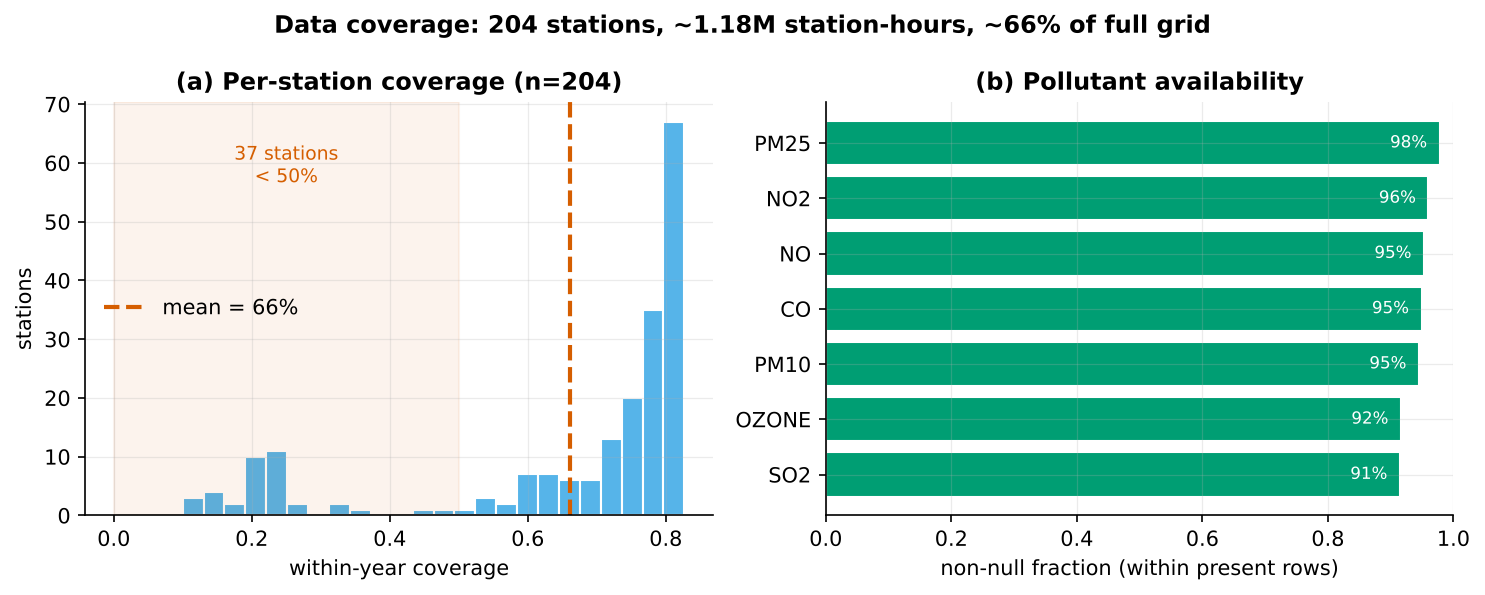
\includegraphics[width=0.98\linewidth]{fig1_network_coverage.png}
  \caption{Network coverage. (a) Distribution of within-year temporal completeness
  across the $204$ stations (mean $66\%$; $37$ stations below $50\%$, shaded).
  (b) Per-pollutant non-null fraction within present station-hours. Geolocation of
  individual monitors is not retained in the public telemetry export and is therefore
  not mapped; the network is urban and spatially concentrated in the National Capital
  Region and major metropolitan centres (a representativeness limitation, \cref{sec:gate}).}
  \label{fig:coverage}
\end{figure}

\subsection{Sanitization}
Three classes of non-physical artifact were identified and flagged. (i) \emph{Instrument
saturation / round caps}: distinct spikes of mass at round ceilings
(NO, NO\textsubscript{2}, O\textsubscript{3} near $500$; PM\textsubscript{2.5} near
$1000$). (ii) \emph{Zero-padding and dropout}: runs of exact zeros and abrupt gaps
inconsistent with ambient variability. (iii) \emph{Non-physical outliers}: $35$ values
exceeding physically plausible bounds were flagged and excluded from distributional
summaries. Screening these artifacts materially changes downstream covariance
estimates---for example, the CO--NO correlation rises from $0.14$ to $0.42$---which is
itself evidence that naive clustering is sensitive to data hygiene (\cref{sec:results}).

\subsection{The unit-provenance discovery}
\label{sec:units}
A pre-registration-style verification of measurement units against the
\emph{authoritative} OpenAQ per-sensor metadata revealed a material provenance defect
(\cref{fig:units}). NO is reported in parts-per-billion (ppb) at every station;
O\textsubscript{3}, PM\textsubscript{2.5} and PM\textsubscript{10} are reported in
mass concentration (\ugm{}) and are unit-consistent. However, CO, NO\textsubscript{2}
and SO\textsubscript{2} carry \emph{duplicate sensors reporting in both ppb and \ugm{}}
at almost every station (CO at $183/198$ stations, NO\textsubscript{2} at $187/199$,
SO\textsubscript{2} at $178/191$), while the exported telemetry retains a single value
per pollutant per station-hour with \emph{no record of which sensor produced it}. A
mixing ratio (ppb) and a mass concentration (\ugm{}) are related only through molecular
weight and ambient temperature and pressure; they are not comparable, and the mix
cannot be reconciled post hoc from the stored data. This supersedes an earlier,
value-based inference (which had suggested a uniform CO regime): the authoritative
sensor metadata governs. Consequently, we restrict all quantitative cross-station
inference to the unit-consistent species (NO, O\textsubscript{3},
PM\textsubscript{2.5}, PM\textsubscript{10}); the two headline results below---ozone
estimation and the NO$\rightarrow$O\textsubscript{3} association---depend only on these.

\begin{figure}[t]
  \centering
  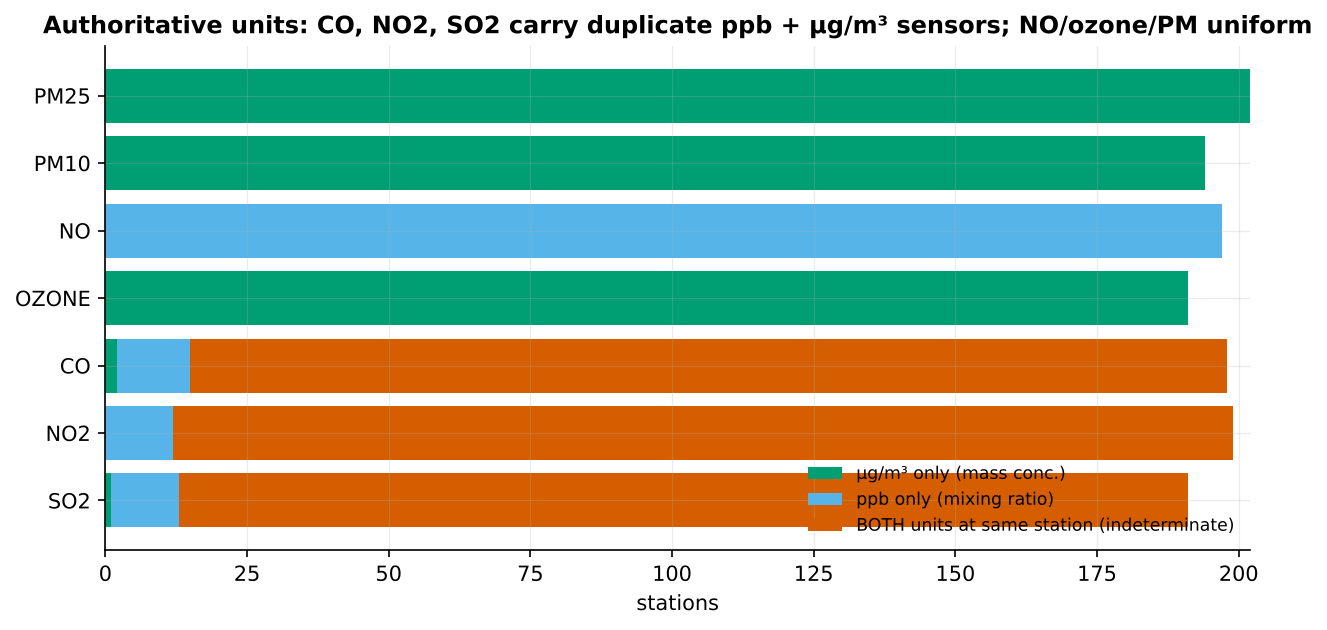
\includegraphics[width=0.92\linewidth]{fig6_units_verification.png}
  \caption{Authoritative unit verification per species. PM\textsubscript{2.5},
  PM\textsubscript{10} and O\textsubscript{3} are uniform \ugm{}; NO is uniform ppb;
  CO, NO\textsubscript{2} and SO\textsubscript{2} carry duplicate ppb and \ugm{}
  sensors at the same station (orange), rendering their stored unit indeterminate.}
  \label{fig:units}
\end{figure}

\subsection{Summary statistics}
\cref{tab:summary} reports distributional summaries of the sanitized telemetry.
Values are in the stored measurement scale; for the unit-indeterminate species
(CO, NO\textsubscript{2}, SO\textsubscript{2}) the magnitudes are not cross-station
comparable and are shown for completeness only. The heavy right skew of
PM\textsubscript{2.5} and PM\textsubscript{10} (large standard deviations, high 95th
percentiles) is characteristic of the Indian urban winter particulate regime.

\begin{table}[t]
  \centering
  \caption{Summary statistics of the sanitized telemetry (calendar year 2025,
  $204$ stations). Missing fraction is relative to present station-hours.
  CO, NO\textsubscript{2}, SO\textsubscript{2} are unit-indeterminate
  (\cref{sec:units}); PM in \ugm{}, O\textsubscript{3} in \ugm{}, NO in ppb.}
  \label{tab:summary}
  \begin{tabular}{lrrrrr}
    \toprule
    Pollutant & Mean & Std.\ dev. & 5th pct. & 95th pct. & Missing frac. \\
    \midrule
    O\textsubscript{3}            & 30.52  & 30.89  & 2.57  & 89.80  & 0.084 \\
    NO                            & 14.81  & 29.13  & 0.88  & 49.20  & 0.047 \\
    NO\textsubscript{2}           & 27.33  & 27.37  & 2.60  & 80.10  & 0.040 \\
    CO                            & 0.87   & 2.40   & 0.10  & 2.18   & 0.051 \\
    SO\textsubscript{2}           & 13.47  & 25.67  & 1.75  & 35.20  & 0.085 \\
    PM\textsubscript{10}          & 121.50 & 116.48 & 18.20 & 349.20 & 0.055 \\
    PM\textsubscript{2.5}         & 58.28  & 73.79  & 6.50  & 185.00 & 0.022 \\
    \bottomrule
  \end{tabular}
\end{table}

\section{Methodology}
\label{sec:methods}

\subsection{Governing physical dynamics}
The ambient concentration field $C_i(\mathbf{x},t)$ of chemical species $i$ evolves
according to the atmospheric advection--diffusion--reaction equation,
\begin{equation}
  \frac{\partial C_i}{\partial t}
  = \underbrace{-\,\nabla \cdot (\mathbf{u}\, C_i)}_{\text{advection}}
  + \underbrace{\nabla \cdot (\mathbf{K}\, \nabla C_i)}_{\text{turbulent diffusion}}
  + \underbrace{R_i(C_1,\dots,C_m,\,T,\,h\nu)}_{\text{chemistry}}
  + \underbrace{E_i(\mathbf{x},t)}_{\text{emissions}},
  \label{eq:adr}
\end{equation}
where $\mathbf{u}(\mathbf{x},t)$ is the wind velocity field, $\mathbf{K}$ the
(second-order) eddy-diffusivity tensor, $R_i$ the net chemical production/loss rate for
species $i$ as a function of all $m$ reacting species, temperature $T$ and the actinic
photon flux $h\nu$, and $E_i$ the surface emission rate. Equation~\eqref{eq:adr} makes
the epistemic gap explicit: a single-site, contemporaneous regression of $C_i$ on the
other $C_j$ and a few meteorological scalars discards the spatial transport operators
entirely, linearizes the strongly non-linear reaction term $R_i$, and---critically---
never observes the emission field $E_i$ on which policy acts. It can estimate a local,
time-averaged \emph{response surface}, not the operator in \eqref{eq:adr}.

\subsection{Predictive formulation and leakage controls}
Let $y_{s,t}$ denote the standardized ozone concentration at station $s$ and hour $t$,
and $\mathbf{x}_{s,t}\in\RR^{d}$ the vector of contemporaneous covariates (the other
six pollutants and four meteorological variables). We estimate $\hat y = f(\mathbf{x})$
with gradient-boosted regression trees \citep{chen2016xgboost}, chosen for their strong
tabular performance under non-linear interactions and implemented within a distributed
Apache Spark pipeline \citep{zaharia2016spark}; hyper-parameters are fixed a priori and
never tuned on any evaluation fold.

Because $y_{s,t}$ is strongly autocorrelated in both time and space, the choice of
evaluation protocol is not a detail but the central inferential control
\citep{kaufman2012leakage,roberts2017cv,varma2006cv}. We contrast three protocols:
\begin{enumerate}
  \item \emph{i.i.d.\ random split} (70/30 over rows): the standard but
  \emph{leaky} baseline, in which near-duplicate neighbouring hours of the same station
  appear in both train and test.
  \item \emph{Blocked temporal holdout}: train on quarters Q1--Q3 (months 1--9),
  evaluate on Q4 (months 10--12). Temporal blocks are never split.
  \item \emph{Spatial leave-stations-out}: $5$-fold \texttt{GroupKFold} with the station
  identifier as the grouping key, so that no station appears in both train and test;
  this probes transfer to \emph{unmonitored} locations.
\end{enumerate}
All preprocessing (standardization, imputation) is fit on the training fold only.
We report against a ladder of reference baselines: (i) \emph{lag-1 persistence},
$\hat y_{s,t}=y_{s,t-1}$; (ii) a \emph{station $\times$ hour $\times$ month
diurnal-seasonal mean}, the strongest purely climatological predictor; and (iii) an
$L_2$-regularized \emph{Ridge} regression \citep{hastie2009esl} on the same covariates,
as a linear reference for the boosted model. Uncertainty is quantified by a station-block bootstrap.

\subsection{Covariance clustering versus bilinear receptor modelling}
The pipeline's first stage groups species by $k$-means over their inter-species
Pearson correlation profiles. It is essential to state precisely what this does
\emph{not} do. Quantitative source apportionment is a bilinear receptor model; positive
matrix factorization (PMF) \citep{paatero1994pmf} factorizes a speciated
concentration matrix $X=[x_{ij}]$ (sample $i$, chemical species $j$) as
\begin{equation}
  x_{ij} = \sum_{k=1}^{p} g_{ik} f_{kj} + e_{ij},
  \qquad g_{ik}\ge 0,\; f_{kj}\ge 0,
  \label{eq:pmf}
\end{equation}
where $g_{ik}$ is the contribution of source $k$ to sample $i$, $f_{kj}$ the
chemical profile of source $k$, and $e_{ij}$ a residual weighted by the measurement
uncertainty $\sigma_{ij}$ through the objective
$Q=\sum_{ij}(e_{ij}/\sigma_{ij})^2$. PMF requires (a) chemically speciated composition
(including organic and elemental carbon and key tracers), (b) per-measurement
uncertainties, and (c) enough species to identify $p$ non-negative factors. Our data
provide only seven criteria pollutants, no speciation, no VOCs, and no per-measurement
uncertainties. $k$-means over criteria-gas correlations is therefore an
\emph{exploratory inter-species covariance clustering}, and its clusters are
mathematically distinct from the latent source factors $\{g_{ik},f_{kj}\}$ of
\eqref{eq:pmf}; they admit no mass-balance or source interpretation.

\subsection{Causal discovery via DirectLiNGAM}
For exploratory structure, we model the standardized pollutant vector
$\zvec\in\RR^{m}$ as a linear, non-Gaussian, acyclic structural equation model,
\begin{equation}
  \zvec = \bmat\,\zvec + \evec,
  \label{eq:sem}
\end{equation}
where $\bmat$ is a strictly lower-triangular (under some causal ordering) matrix of
structural coefficients and $\evec$ is a vector of mutually independent, non-Gaussian
exogenous disturbances. Unlike constraint-based
discovery \citep{spirtes2000causation}, DirectLiNGAM
\citep{shimizu2006lingam,shimizu2011directlingam} estimates a causal ordering and the
coefficients $\bmat$ directly, exploiting non-Gaussianity to orient edges; non-linear
generalizations exist via additive-noise models \citep{hoyer2009anm} but inherit the
same confounding sensitivity. Its validity rests on four assumptions:
(A1) \emph{acyclicity} of the generating graph; (A2) \emph{linearity} of the structural
equations; (A3) \emph{non-Gaussian} disturbances with non-zero variance; and
(A4) \emph{causal sufficiency}---no unobserved common causes of two or more observed
variables. We encode domain knowledge as a prior-knowledge constraint matrix
$K\in\{0,1,{-}1\}^{m\times m}$ that forbids edges from secondary pollutants
(e.g.\ O\textsubscript{3}) into primary combustion tracers (e.g.\ NO, CO), consistent
with emission chemistry. Edge reliability is assessed by a station-block bootstrap
(reporting per-edge selection frequency and coefficient sign), and---decisively---by
refitting with the meteorological variables included as exogenous nodes, which tests
assumption (A4) against the dominant confounder.

\subsection{Analytical derivation of the global Pareto frontier}
The optimization stage searches, with the NSGA-II evolutionary algorithm
\citep{deb2002nsga2} as implemented in the Optuna framework \citep{akiba2019optuna},
for policies minimizing two standardized objectives built from the fitted linear
response surface. Empirically the fitted surface is
\begin{align}
  z_{\mathrm{O_3}}   &= \alpha\, z_{\mathrm{NO}}, & \alpha &< 0, \label{eq:resp_o3}\\
  z_{\mathrm{PM_{2.5}}} &= \beta_1 z_{\mathrm{NO}} + \beta_2 z_{\mathrm{NO_2}}
                            + \beta_3 z_{\mathrm{CO}}, & \beta_1,\beta_2,\beta_3 &> 0,
  \label{eq:resp_pm}
\end{align}
with fitted values $\alpha=-0.124$, $\beta_1=0.092$, $\beta_2=0.219$, $\beta_3=0.228$;
SO\textsubscript{2} and VOC enter with zero coefficient (VOC is not a fitted variable),
so the effective decision vector is
$\mathbf{z}=(z_{\mathrm{NO}},z_{\mathrm{NO_2}},z_{\mathrm{CO}})$ over the search
hypercube $z_j\in[z_{\min},z_{\max}]=[-2,0]$ (reductions only, bounded at $-2\sigma$).

\begin{lemma}[Collapse of the linear Pareto front]
\label{lem:pareto}
Consider the bi-objective minimization of
$\big(f_1(\mathbf{z}),f_2(\mathbf{z})\big)=\big(z_{\mathrm{O_3}},z_{\mathrm{PM_{2.5}}}\big)$
defined by \eqref{eq:resp_o3}--\eqref{eq:resp_pm} over
$\mathbf{z}\in[z_{\min},z_{\max}]^3$ with $\alpha<0$ and $\beta_1,\beta_2,\beta_3>0$.
Then every Pareto-optimal point satisfies
$z_{\mathrm{NO_2}}^{\star}=z_{\mathrm{CO}}^{\star}=z_{\min}$, and the Pareto set is the
one-dimensional segment
\[
  \mathcal{P}=\Big\{\big(z_{\mathrm{NO}},z_{\min},z_{\min}\big)\;:\;
  z_{\mathrm{NO}}\in[z_{\min},z_{\max}]\Big\},
\]
whose image is the line segment
$z_{\mathrm{PM_{2.5}}} = \tfrac{\beta_1}{\alpha}\,z_{\mathrm{O_3}}
+(\beta_2+\beta_3)\,z_{\min}$.
\end{lemma}

\begin{proof}
The objective $f_1$ depends only on $z_{\mathrm{NO}}$, while $f_2$ is strictly
increasing in each of $z_{\mathrm{NO_2}}$ and $z_{\mathrm{CO}}$ (as $\beta_2,\beta_3>0$)
and does not appear in $f_1$. Fix any feasible point $\mathbf{z}$ with
$z_{\mathrm{NO_2}}>z_{\min}$. The point $\mathbf{z}'$ obtained by lowering
$z_{\mathrm{NO_2}}$ to $z_{\min}$ (all else equal) is feasible, leaves $f_1$ unchanged,
and strictly decreases $f_2$; hence $\mathbf{z}'$ dominates $\mathbf{z}$, so $\mathbf{z}$
is not Pareto-optimal. The identical argument applies to $z_{\mathrm{CO}}$. Therefore
every Pareto-optimal point has $z_{\mathrm{NO_2}}^{\star}=z_{\mathrm{CO}}^{\star}=z_{\min}$.

Restricted to this face the objectives reduce to
$f_1=\alpha z_{\mathrm{NO}}$ and
$f_2=\beta_1 z_{\mathrm{NO}} + (\beta_2+\beta_3)z_{\min}$. Since $\alpha<0$, $f_1$ is
strictly decreasing in $z_{\mathrm{NO}}$, whereas $f_2$ is strictly increasing in
$z_{\mathrm{NO}}$ (as $\beta_1>0$); the two objectives are therefore in strict conflict
along $z_{\mathrm{NO}}$, so no interior point of the segment dominates another and the
entire segment is Pareto-optimal. Eliminating $z_{\mathrm{NO}}=f_1/\alpha$ gives
$f_2=\tfrac{\beta_1}{\alpha}f_1+(\beta_2+\beta_3)z_{\min}$, a straight line.
\end{proof}

\begin{corollary}
\label{cor:pareto}
The true Pareto frontier of the fitted linear surrogate is a closed-form line segment
computable without any metaheuristic search. Any evolutionary approximation can at best
match it and, lacking the boundary structure of \cref{lem:pareto}, will generically
return interior, dominated points.
\end{corollary}

\paragraph{Benchmark metrics.}
Let $\mathcal{F}$ be a dense discretization of the exact frontier $\mathcal{P}$ and
$A=\{\mathbf{a}_k\}_{k=1}^{n}$ the archive of heuristic solutions in objective space.
The \emph{generational distance} is
\begin{equation}
  \mathrm{GD}(A)=\Big(\frac{1}{n}\sum_{k=1}^{n} d_k^{2}\Big)^{1/2},
  \qquad d_k=\min_{\mathbf{p}\in\mathcal{F}}\lVert \mathbf{a}_k-\mathbf{p}\rVert_2 ,
  \label{eq:gd}
\end{equation}
and, for a shared reference point $\mathbf{r}$ dominated by all points, the
\emph{hypervolume error} is
\begin{equation}
  \mathrm{HVE}=\frac{\mathrm{HV}(\mathcal{F};\mathbf{r})-\mathrm{HV}(A;\mathbf{r})}
  {\mathrm{HV}(\mathcal{F};\mathbf{r})},
  \label{eq:hve}
\end{equation}
where $\mathrm{HV}(\cdot\,;\mathbf{r})$ is the dominated hypervolume \citep{zitzler1999hv}.
$\mathrm{GD}=0$ and $\mathrm{HVE}=0$ iff the archive lies on the true frontier.

\section{Results}
\label{sec:results}

\subsection{Predictive benchmarking and the cost of leakage}
\cref{tab:bench} reports contemporaneous ozone estimation across the three evaluation
protocols and the baseline ladder. The result is unambiguous: apparent skill is an
artifact of the protocol. The gradient-boosted model attains $R^2=0.412$ under the
i.i.d.\ random split, but this collapses to $R^2=0.251$ under the blocked temporal Q4
holdout and $R^2=0.304$ under spatial leave-stations-out, falling further to
$R^2=0.219$ under the strict temporal$\times$spatial intersection
(\cref{fig:leakage}). The $\sim$$0.16$--$0.19$ absolute $R^2$ gap between the random
split and the blocked/grouped protocols is pure spatio-temporal leakage: neighbouring
hours of the same station, near-duplicates of one another, leak across the random
train/test boundary \citep{kaufman2012leakage,roberts2017cv}.

Two baselines frame the honest skill. The linear Ridge reference is weak everywhere
($R^2\le 0.17$), confirming that the signal the boosted model captures is genuinely
non-linear; but a trivial \emph{lag-1 persistence} predictor attains $R^2=0.794$ on the
same temporal holdout. The learned model is thus valuable only where persistence is
unavailable---namely spatial interpolation to unmonitored sites---and is \emph{beaten
by doing nothing} for temporal gap-filling. The diurnal-seasonal climatology
($R^2=0.041$) shows that static station behaviour alone explains almost none of the
hour-to-hour variance.

\begin{table}[t]
  \centering
  \caption{Leakage-safe predictive benchmarking of contemporaneous ozone estimation.
  All preprocessing fit on the training fold only; hyper-parameters fixed a priori.
  Persistence and the diurnal-seasonal mean are defined only for the temporal
  holdout. Lower RMSE/MAE and higher $R^2$ are better.}
  \label{tab:bench}
  \begin{tabular}{llrrr}
    \toprule
    Protocol & Model & $R^2$ & RMSE & MAE \\
    \midrule
    \multirow{2}{*}{Random split (leaky)}
      & XGBoost                       & 0.412 & 23.72 & 14.90 \\
      & Ridge ($L_2$)                 & 0.167 & 28.21 & 18.63 \\
    \midrule
    \multirow{4}{*}{Blocked temporal (Q1--Q3 $\to$ Q4)}
      & XGBoost                       & 0.251 & 26.49 & 16.19 \\
      & Ridge ($L_2$)                 & 0.082 & 29.32 & 18.78 \\
      & Diurnal-seasonal mean         & 0.041 & 29.98 & 20.04 \\
      & Persistence (lag-1)           & \textbf{0.794} & \textbf{13.88} & \textbf{5.57} \\
    \midrule
    \multirow{2}{*}{Spatial leave-stations-out (5-fold)}
      & XGBoost                       & 0.304 & 27.94 & 18.45 \\
      & Ridge ($L_2$)                 & 0.159 & 28.33 & 18.73 \\
    \midrule
    Temporal $\times$ spatial (strict)
      & XGBoost                       & 0.219 & 30.00 & 18.41 \\
    \bottomrule
  \end{tabular}
\end{table}

\begin{figure}[t]
  \centering
  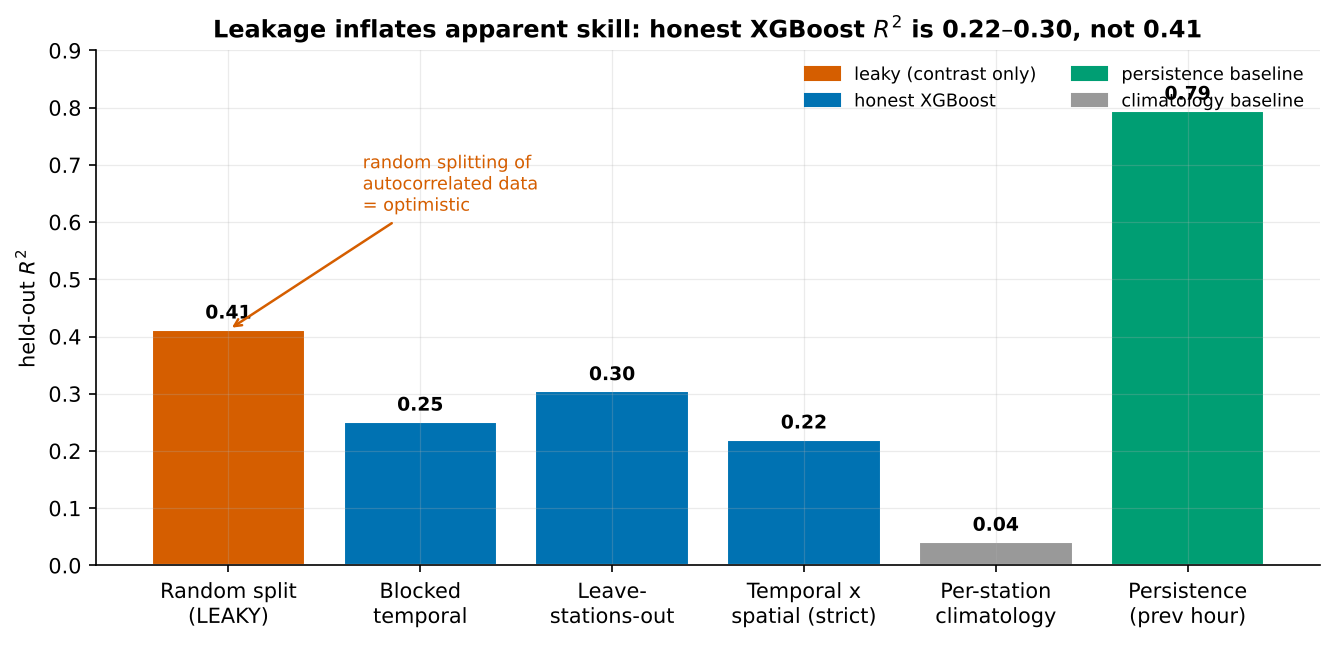
\includegraphics[width=0.95\linewidth]{fig2_leakage_benchmark.png}
  \caption{Held-out $R^2$ for contemporaneous ozone by evaluation protocol. Random
  splitting of autocorrelated telemetry inflates skill to $0.41$; honest blocked and
  grouped protocols give $0.22$--$0.30$. A previous-hour persistence baseline (green)
  dominates for temporal gap-filling.}
  \label{fig:leakage}
\end{figure}

\subsection{Meteorology ablation}
Stripping covariate groups under the blocked temporal protocol isolates their
contributions. A weather-only model attains $R^2=0.140$ and a pollutant-only model
$R^2=0.132$, while the full model reaches $R^2=0.251$. The incremental value of the six
pollutants \emph{beyond} meteorology is therefore only $\Delta R^2\approx+0.117$: most
of the explainable ozone variance is meteorological, and the chemical covariates add a
small, though non-trivial, increment. Any downstream ``mechanistic'' reading must
account for the fact that meteorology, not chemistry, carries the bulk of the signal.

\subsection{Recovered structure and its atmospheric interpretation}
The bootstrap-stabilized DirectLiNGAM structure is shown in \cref{fig:dag}. Of all
candidate edges, exactly one is both bootstrap-stable (selection frequency $1.0$) and
survives the inclusion of meteorology as exogenous nodes: the negative edge
$\mathrm{NO}\rightarrow\mathrm{O_3}$, with standardized coefficient
$-0.138\pm0.007$ in the pollutant-only model, attenuating to $-0.108$ once temperature,
humidity, wind and pressure are included. This is the chemical signature of
\emph{localized} titration, $\mathrm{NO}+\mathrm{O_3}\rightarrow\mathrm{NO_2}+\mathrm{O_2}$,
expected in fresh, NO-rich urban (traffic-dominated) air \citep{sillman1999,
monks2015ozone}: ambient NO destroys ozone locally. Crucially, this is \emph{not}
regional photochemical production, which is governed by VOC oxidation that these data
cannot observe. The remaining high-frequency edges
($\mathrm{NO}\rightarrow\mathrm{NO_2}$, $+0.40$; $\mathrm{NO_2}\rightarrow\mathrm{PM_{2.5}}$,
$+0.23$; and the CO combustion edges, frequency $0.91$) are consistent with shared
combustion co-emission but involve unit-indeterminate species (\cref{sec:units}) and,
for the particulate edges, collapse once meteorology is included---evidence that the
pollutant-only graph is confounded by the boundary layer (\cref{sec:gate}).
SO\textsubscript{2} edges are unstable (frequency $\le0.5$) and are not retained.

\begin{figure}[t]
  \centering
  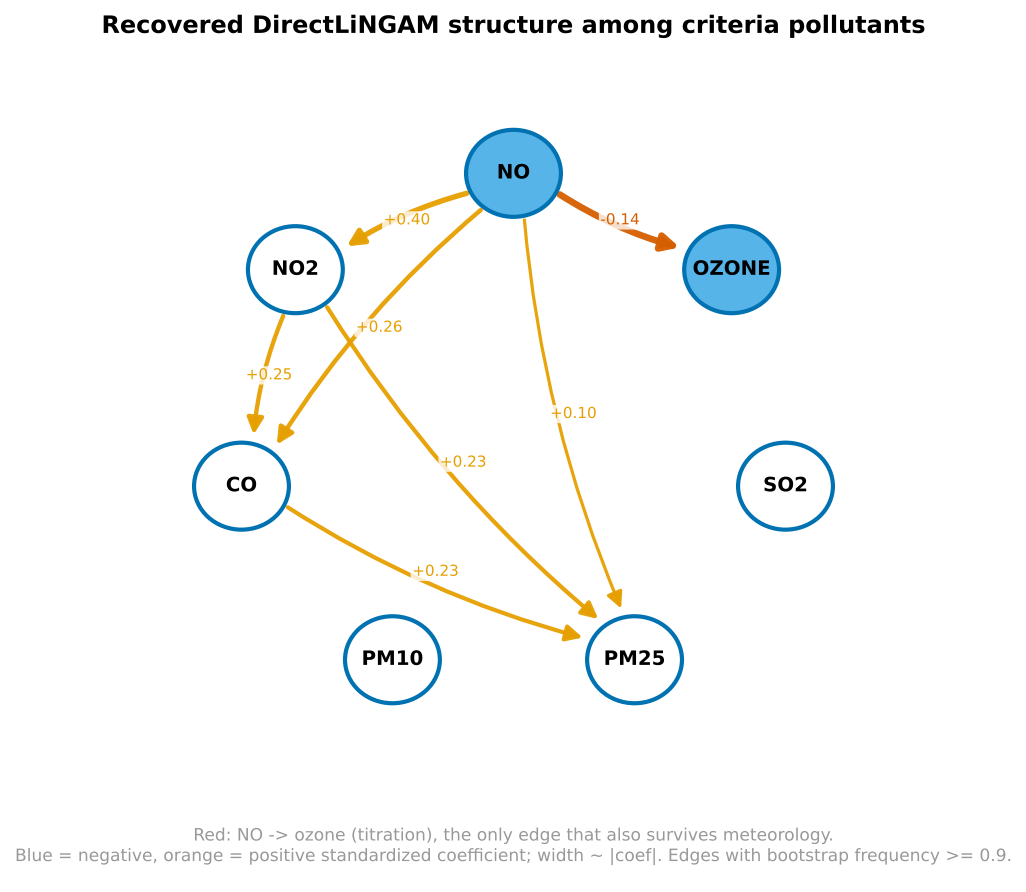
\includegraphics[width=0.78\linewidth]{fig3_causal_dag.png}
  \caption{Recovered DirectLiNGAM structure (bootstrap frequency $\ge 0.9$). Only
  $\mathrm{NO}\rightarrow\mathrm{O_3}$ (red, negative) is both stable and robust to
  meteorological confounding. Edge width scales with $|$coefficient$|$;
  SO\textsubscript{2} carries no stable edge.}
  \label{fig:dag}
\end{figure}

\subsection{Empirical Pareto frontier versus the NSGA-II archive}
\cref{lem:pareto} predicts that the true frontier is a one-dimensional segment with
$z_{\mathrm{NO_2}}=z_{\mathrm{CO}}=z_{\min}$. We computed this exact segment in closed
form and audited the $19$ saved NSGA-II candidate policies against it
(\cref{tab:pareto}, \cref{fig:pareto}). Every one of the $19$ heuristic policies is
dominated by the exact frontier---a $100\%$ dominance rate---with a mean objective-space
gap of $0.046$ (maximum $0.298$) in standardized PM\textsubscript{2.5}, a generational
distance of $\mathrm{GD}=0.084$ \eqref{eq:gd}, and a hypervolume error of
$\mathrm{HVE}=6.6\%$ \eqref{eq:hve}. The heuristic fails precisely as
\cref{cor:pareto} anticipates: unaware of the boundary structure, NSGA-II scatters
interior points rather than driving the reducible coordinates to their bound. For a
linear surrogate, the metaheuristic is not merely unnecessary---it is strictly inferior
to a closed-form solution that any analyst can write down.

\begin{table}[t]
  \centering
  \caption{Audit of the heuristic NSGA-II archive against the exact analytical Pareto
  frontier of the fitted linear surrogate (\cref{lem:pareto}). Objectives are
  standardized; gaps are Euclidean in objective space.}
  \label{tab:pareto}
  \begin{tabular}{lr}
    \toprule
    Quantity & Value \\
    \midrule
    Heuristic candidate policies audited          & $19$ \\
    Policies dominated by the exact frontier       & $19$ ($100\%$) \\
    Mean gap to frontier (std.\ PM\textsubscript{2.5}) & $0.046$ \\
    Maximum gap to frontier                        & $0.298$ \\
    Generational distance, $\mathrm{GD}$           & $0.084$ \\
    Hypervolume error, $\mathrm{HVE}$              & $6.6\%$ \\
    Exact frontier: $z_{\mathrm{NO_2}}^\star=z_{\mathrm{CO}}^\star$ & $z_{\min}=-2$ \\
    Exact frontier endpoints $(z_{\mathrm{O_3}},z_{\mathrm{PM_{2.5}}})$
      & $(0,-0.89)\to(0.25,-1.08)$ \\
    \bottomrule
  \end{tabular}
\end{table}

\begin{figure}[t]
  \centering
  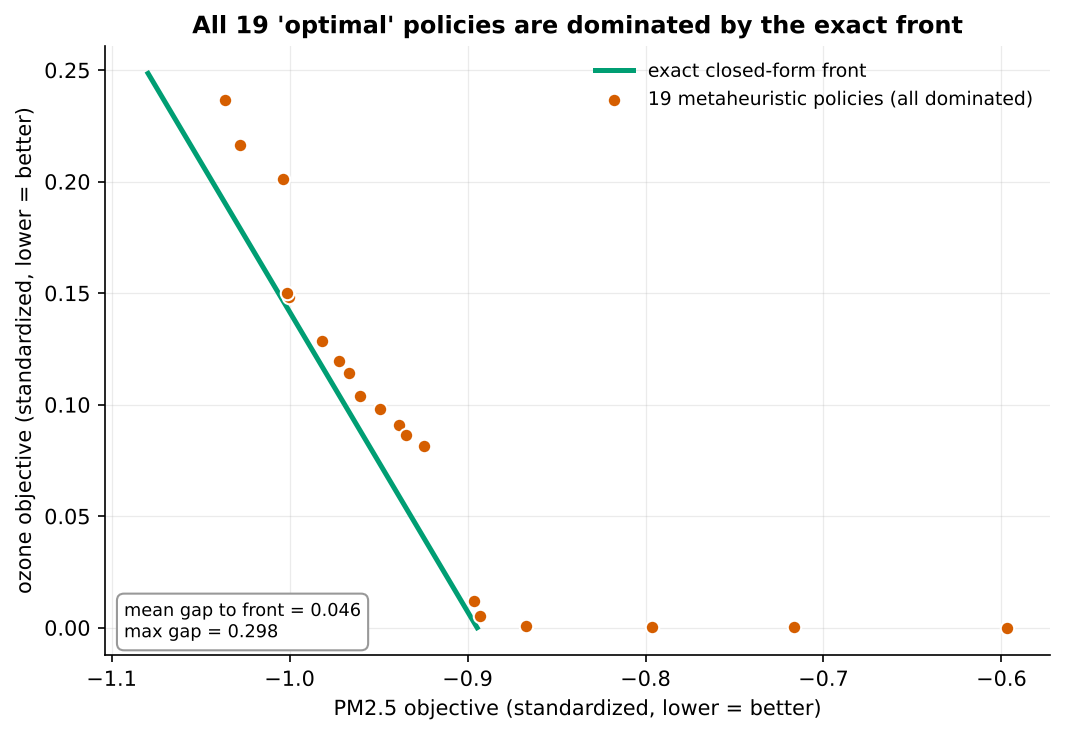
\includegraphics[width=0.72\linewidth]{fig4_analytic_pareto.png}
  \caption{The $19$ NSGA-II ``optimal'' policies (orange) against the exact closed-form
  Pareto frontier (green) of the linear surrogate. All heuristic points are dominated.}
  \label{fig:pareto}
\end{figure}

\subsection{Model explainability}
\cref{fig:shap} shows the global SHAP importance ranking \citep{lundberg2017shap,
lundberg2020treeshap} for the ozone model. Relative humidity and temperature dominate,
followed by NO as the leading chemical covariate---mirroring both the meteorology
ablation and the single stable structural edge. We stress the epistemic status of this
agreement: SHAP and DirectLiNGAM are two summaries of the \emph{same} fitted model and
data. Their concordance on the sign and prominence of NO is \emph{internal
consistency}, not independent validation; it cannot license a causal claim that the
leakage-safe and confounding analyses do not already support.

\begin{figure}[t]
  \centering
  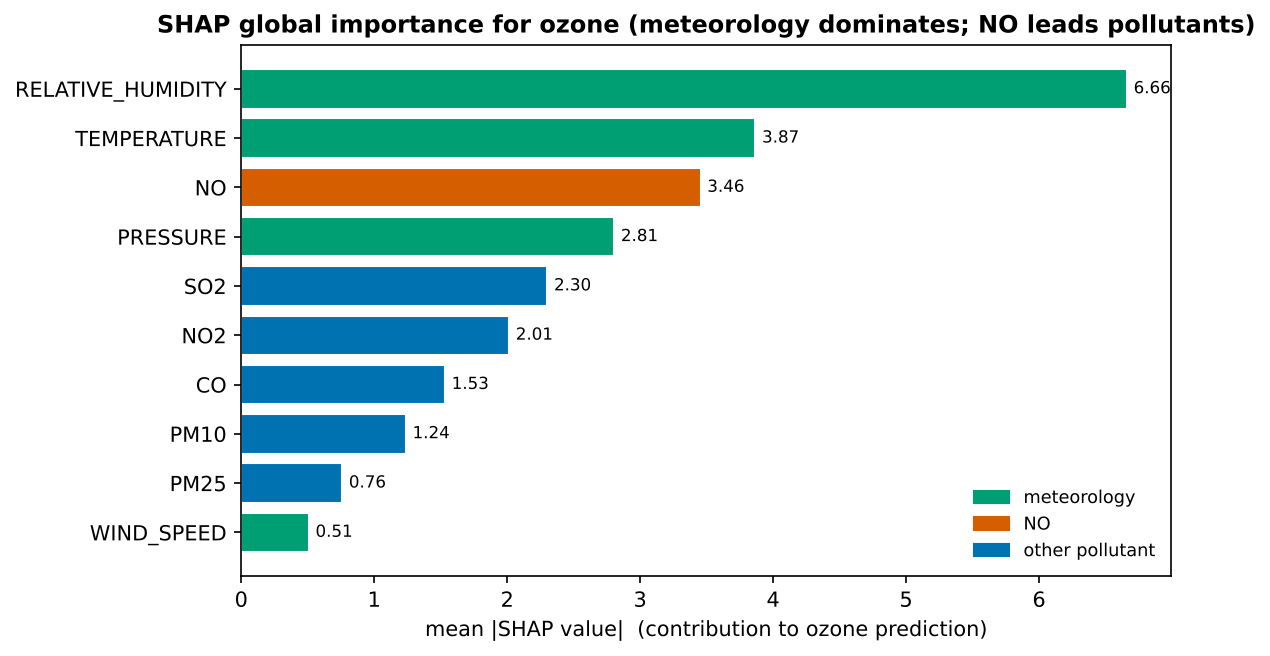
\includegraphics[width=0.9\linewidth]{fig5_shap_importance.png}
  \caption{Global SHAP importance (mean $|$SHAP$|$) for ozone estimation. Meteorology
  dominates; NO is the leading chemical covariate, consistent with
  \cref{fig:dag}. Per-sample attributions were not retained, so a beeswarm is not shown.}
  \label{fig:shap}
\end{figure}

\section{Discussion: A Scientific Identification Gate}
\label{sec:gate}

The audit in \cref{sec:results} is not a catalogue of incidental shortcomings; the
three findings share a common root. A pooled, linear, observational model of ambient
telemetry cannot, in principle, answer the interventional and apportionment questions
the original pipeline posed. We formalize this as a four-part \emph{identification
gate}: criteria that an observational air-quality analysis must pass before causal,
apportionment or policy language is warranted.

\subsection{Gate 1: structural absence of VOCs}
Ozone sensitivity is governed by the VOC-to-NO$_x$ ratio
\citep{sillman1999,monks2015ozone,seinfeld2016atmospheric}. Without continuous
hydrocarbon speciation---or an observational proxy such as the formaldehyde-to-NO$_2$
column ratio (HCHO/NO\textsubscript{2}) from satellite retrievals---the VOC-limited and
NO$_x$-limited regimes are empirically indistinguishable in these data. A model that
never observes VOCs cannot resolve which regime produced a given ozone value, and so
cannot attribute an ozone change to a precursor intervention. Our single recovered
edge, $\mathrm{NO}\rightarrow\mathrm{O_3}<0$, is consistent with this limitation: it is
the \emph{titration} term, the one piece of ozone chemistry that does not require
observing VOCs, and it must not be generalized to regional photochemical production.

\subsection{Gate 2: unobserved planetary-boundary-layer confounding}
The diurnal cycle of the planetary boundary layer (PBL) is a powerful \emph{unobserved
common cause}. At night and in winter the PBL collapses, trapping fresh emissions in a
shallow volume and simultaneously raising the measured concentrations of all primary,
co-emitted species; by day it deepens and dilutes them together. This single latent
variable induces strong positive correlations among co-emitted pollutants that have
nothing to do with any direct inter-pollutant causal mechanism, violating the causal
sufficiency assumption (A4) of \eqref{eq:sem}. The empirical signature is exactly what
we observe: the particulate and combustion edges of \cref{fig:dag} are stable in the
pollutant-only graph but collapse once meteorological proxies of mixing are included.
A spuriously ``discovered'' $\mathrm{CO}\rightarrow\mathrm{PM_{2.5}}$ edge is better read
as two species responding to a common, unmeasured mixing volume. Mitigation requires
either direct PBL-height observations or explicit meteorological deconfounding
\citep{grange2019metnorm,grange2018rf,chernozhukov2018double}.

\subsection{Gate 3: the concentration--emission fallacy}
This is the decisive gate for policy. The optimizer of \cref{lem:pareto} acts on
\emph{standardized ambient concentrations}: a recommendation such as
``$z_{\mathrm{NO_2}}=z_{\min}=-2\sigma$'' is a point on a correlational surface, not an
emission control. Two failures follow. First, there is no validated map from this
concentration vector back to a feasible set of sectoral emission reductions; the
inverse problem is precisely the ill-posed source attribution that
\eqref{eq:adr} would have to solve. Second, the search can select physically
impossible states: for a right-skewed, non-negative pollutant whose standardized mean
sits near zero, a target of $-2\sigma$ can correspond to a \emph{negative physical
mass concentration}. Formally, if $C=\mu+\sigma z$ with $\mu\lesssim 2\sigma$ (as holds
for several species in \cref{tab:summary}), then $z=-2$ implies $C<0$. An
``optimal policy'' that prescribes negative pollutant mass is a reductio: it exposes
that the objective never encoded emissions, feasibility, or benefit. Optimizing a
concentration response surface and reporting the result as a control strategy is a
category error, independent of which optimizer is used.

\subsection{Gate 4: leakage-aware evaluation}
Finally, no skill claim survives without an autocorrelation-aware protocol. As
\cref{tab:bench} shows, the same model and data yield $R^2$ from $0.41$ to $0.22$
depending solely on the split. Random $k$-fold over rows of spatio-temporal telemetry
is not a valid estimate of out-of-sample skill \citep{roberts2017cv,kaufman2012leakage};
blocked-temporal and leave-groups-out protocols, benchmarked against persistence and
climatology, are the minimum standard.

\subsection{Recommendations}
For researchers and regulators deploying observational environmental AI we recommend:
(i) report blocked and grouped validation with persistence and climatology baselines,
never a single random-split number; (ii) treat discovered graphs as hypotheses and test
every edge against meteorological confounding and bootstrap stability before any causal
language; (iii) verify measurement units and provenance against authoritative sensor
metadata, not value heuristics; (iv) reserve ``source apportionment'' for receptor
models \eqref{eq:pmf} with speciation and uncertainties; and (v) never present an
optimizer over ambient concentrations as an emission-control recommendation without a
validated, feasibility-constrained emissions-to-concentrations model.

\section{Conclusion}
\label{sec:conclusion}

We audited a complete prediction-to-policy air-quality pipeline on $1{,}180{,}551$
station-hours from $204$ Indian urban monitors and found that its most consequential
claims do not survive scrutiny. Empirically, spatio-temporal autocorrelation inflates
apparent predictive skill from an honest $R^2\approx0.22$--$0.30$ to a leaky $0.41$,
and the learned model is beaten by trivial persistence for temporal gap-filling;
pollutants add only $\Delta R^2\approx0.12$ beyond meteorology. Structurally, linear
causal discovery recovers a single robust edge---localized NO--O\textsubscript{3}
titration---rather than any regional photochemical mechanism, a ceiling imposed by the
structural absence of VOCs and sharpened by a verified ppb/\ugm{} unit-provenance
defect in three species. Algorithmically, we proved (\cref{lem:pareto}) that the true
Pareto frontier of the fitted linear surrogate is a closed-form line segment, against
which $100\%$ of the heuristic NSGA-II policies are dominated
($\mathrm{GD}=0.084$, $\mathrm{HVE}=6.6\%$).

Taken together these results motivate the four-part identification gate of
\cref{sec:gate} and a deliberate reframing. Rather than an over-claimed causal
source-apportionment and control-optimization system, the artifact is most honestly
and usefully released as an \emph{open, leakage-safe benchmark} for multi-pollutant
air-quality machine learning: a real national-scale dataset, a reproducible
evaluation protocol, a baseline ladder that future methods must beat, one
chemically interpretable hypothesis, and an explicit account of what each stronger
claim would require. All code, data, seeds and analysis scripts are released to this
end.

\paragraph{Future work.}
The productive path forward couples, rather than replaces, mechanism and data. We see
three directions: (i) \emph{hybrid modelling}, in which distributed observational
surrogates are coupled to, and constrained by, regional three-dimensional chemical
transport models (e.g.\ WRF-Chem, CMAQ) so that interventions are simulated through
\eqref{eq:adr} rather than fit on a correlational surface; (ii) \emph{speciation},
through low-cost VOC and carbonaceous-aerosol sensor arrays or satellite
HCHO/NO\textsubscript{2} proxies, to pass Gate~1 and enable genuine ozone-regime and
receptor-model analysis; and (iii) \emph{identified causal inference}, using documented
interventions or natural experiments with meteorological deconfounding and
pre-registered estimands. Until an analysis passes the identification gate, the
responsible contribution of observational environmental AI is a well-evaluated
predictive baseline and an honest map of its own limits.

\section*{Acknowledgements}
We thank the Central Pollution Control Board and the OpenAQ and Open-Meteo projects for
maintaining the open data infrastructure that made this audit possible.

\section*{Author contributions}
S.~Krishiykeishav, Pratyush Amit Sharma, Shreerag Venugopalan Nair, Jayshil Vinodbhai
Prajapati and Ryan Vinod jointly designed the study, implemented the pipeline and
audit, and wrote the manuscript.


% ---- back matter ----------------------------------------------------------
\section*{Reproducibility statement}
All code, the committed telemetry dataset, fixed random seeds, per-phase
manifests, and the scripts that regenerate every number, table and figure in
this manuscript are available in the project repository on the
\texttt{review/scientific-audit} branch. Every result is reproducible offline
without a cluster; the audit scripts fix \texttt{SEED = 42}.

\section*{Data availability}
Ambient measurements were obtained from the OpenAQ v3 API \citep{openaq};
meteorological reanalysis from Open-Meteo \citep{openmeteo}. Derived analysis
artifacts are committed to the repository.

\bibliographystyle{plainnat}
\bibliography{references}

\end{document}
